\section{Incremental PID controller}
The discrete PID controller is defined as follows:
\begin{equation}
    u(n)=k_p e(n)+k_i\sum_{k=0}^{n}e(k)+k_d[e(n)-e(n-1)]
\end{equation}
In order to switch to the incremental PID controller expression,
\begin{equation}
    \Delta u(n)=u(n)-u(n-1)
\end{equation}
is defined. Plugging in the controller results in,
\begin{equation}
\begin{split}
    \Delta u(n)&=u(n)-u(n-1)\\
    &=k_p e(n)+k_i\sum_{k=0}^{n}e(k)+k_d[e(n)-e(n-1)]-k_p e(n-1)\\
     &-k_i\sum_{k=0}^{n-1}e(k)-k_d[e(n-1)-e(n-2)]\\
    &=k_p e(n)+k_i\sum_{k=0}^{n-1}e(k)+k_ie(n)+k_de(n)-k_de(n-1)\\
    &-k_p e(n-1)-k_i\sum_{k=0}^{n-1}e(k-1)-k_de(n-1)+k_de(n-2)\\
    &=k_p e(n)-k_p e(n-1)+k_ie(n)+k_de(n)-2k_de(n-1)+k_de(n-2)\\
    &=k_p [e(n)-e(n-1)]+k_ie(n)+k_d[e(n)-2e(n-1)+e(n-2)]
\end{split}
\end{equation}

\section{Fuzzy PI controller}
Let the inputs be $e(n)$ and $\Delta e(n)$ and the output be $\Delta u(n)$ defined as error, change in error and change in control signal, respectively. 

\begin{figure}[h!]
\centering
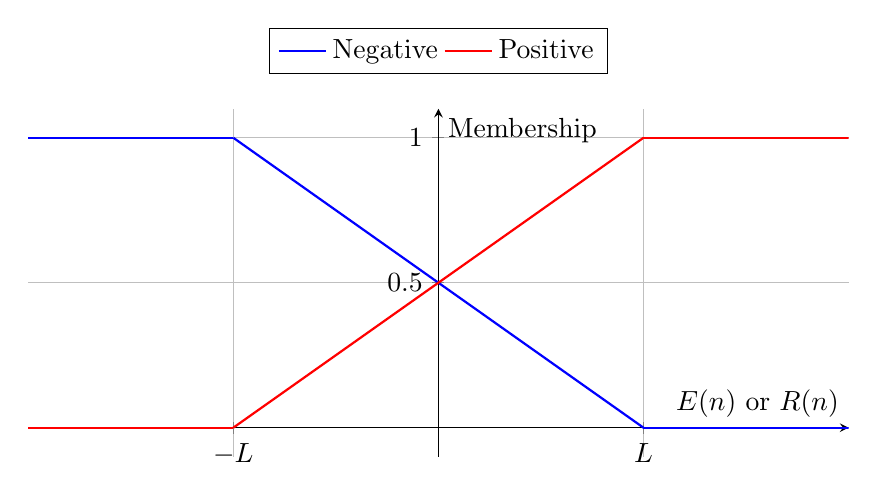
\begin{tikzpicture}
\begin{axis}[
    axis lines=middle,
    xlabel={$E(n)$ or $R(n)$},
    ylabel={Membership},
    ymin=-0.1, ymax=1.1,
    xmin=-20, xmax=20,
    xtick={-10, 0, 10},
    xticklabels={$-L$, $0$, $L$},
    ytick={0, 0.5, 1},
    grid=both,
    width=12cm, height=6cm,
    legend style={at={(0.5,1.1)}, anchor=south, legend columns=-1}
]

% -------- Negative MF (blue) --------
\addplot[domain=-20:-10, thick, blue, samples=2, forget plot] {1};
\addplot[domain=-10:10, thick, blue, samples=100] {(-x + 10)/20};
\addlegendentry{Negative}
\addplot[domain=10:20, thick, blue, samples=2, forget plot] {0};

% -------- Positive MF (red) --------
\addplot[domain=-20:-10, thick, red, samples=2, forget plot] {0};
\addplot[domain=-10:10, thick, red, samples=100] {(x + 10)/20};
\addlegendentry{Positive}
\addplot[domain=10:20, thick, red, samples=2, forget plot] {1};

\end{axis}
\end{tikzpicture}
\caption{Input fuzzy sets: Negative and Positive}
\label{fig:fig1}
\end{figure}
The membership functions Positive(P) and Negative(N) are defined as 
\begin{equation}
    \mu_P(e)\begin{cases}
        0,& e<-L\\
        \frac{e+L}{2L},& -L\leq e\leq L\\
        1,& e>L\\
    \end{cases}\quad
    \mu_N(e)\begin{cases}
        1,& e<-L\\
        \frac{-e+L}{2L},& -L\leq e\leq L\\
        0,& e>L\\
    \end{cases}
\end{equation}
and 
\begin{equation}
    \mu_P(\Delta e)\begin{cases}
        0,& \Delta e<-L\\
        \frac{\Delta e+L}{2L},& -L\leq \Delta e\leq L\\
        1,& \Delta e>L\\
    \end{cases}\quad
    \mu_N(\Delta e)\begin{cases}
        1,& \Delta e<-L\\
        \frac{-\Delta e+L}{2L},& -L\leq \Delta e\leq L\\
        0,& \Delta e>L\\
    \end{cases}
\end{equation}
and depicted in Figure~\ref{fig:fig1}. The membership functions are chosen such that, 
\begin{equation}
    \mu_N(e)+\mu_P(e)=1\quad \mu_N(\Delta e)+\mu_P(\Delta e)=1
\end{equation}

For the output variable the membership function is chosen as
\begin{equation}
    \mu_N(\Delta u)\begin{cases}
        1,& \Delta u=-H\\
        0,& \Delta u\neq-H\\
    \end{cases}\quad
    \mu_P(\Delta u)\begin{cases}
        1,& \Delta u=H\\
        0,& \Delta u\neq H\\
    \end{cases}\quad
    \mu_Z(\Delta u)\begin{cases}
        1,& \Delta u=0\\
        0,& \Delta u\neq 0\\
    \end{cases}
\end{equation}
and is depicted in Figure~\ref{fig:fig2}.
\begin{figure}[h!]
\centering
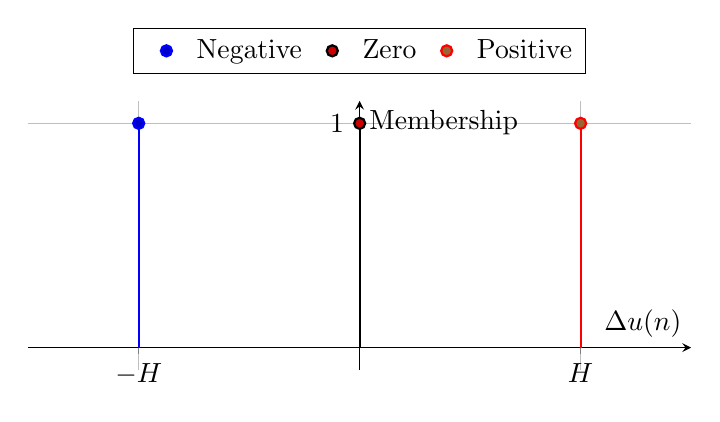
\begin{tikzpicture}
\begin{axis}[
    axis lines=middle,
    xlabel={$\Delta u(n)$},
    ylabel={Membership},
    ymin=-0.1, ymax=1.1,
    xmin=-15, xmax=15,
    xtick={-10, 0, 10},
    xticklabels={$-H$, $0$, $H$},
    ytick={0, 1},
    grid=both,
    width=10cm, height=5cm,
    legend style={at={(0.5,1.1)}, anchor=south, legend columns=-1}
]

% Singleton at -H (Negative)
\addplot+[ycomb, thick, blue, mark=*] coordinates {(-10,1)};
\addlegendentry{Negative}

% Singleton at 0 (Zero)
\addplot+[ycomb, thick, black, mark=*] coordinates {(0,1)};
\addlegendentry{Zero}

% Singleton at +H (Positive)
\addplot+[ycomb, thick, red, mark=*] coordinates {(10,1)};
\addlegendentry{Positive}

\end{axis}
\end{tikzpicture}
\caption{Output fuzzy sets as singleton values at $-H$, $0$, and $H$}
\label{fig:fig2}
\end{figure}

\clearpage
\renewcommand{\arraystretch}{1.5} % Vertical padding
The following rule set is constructed.
\begin{table}[h!]
\centering
\caption{Fuzzy Rule Table: Control Output $\Delta u(n)$ based on Error $e(n)$ and Change of Error $\Delta e(n)$}
\begin{tabular}{c@{\hspace{1em}}|@{\hspace{1em}}c@{\hspace{1em}}c@{\hspace{1em}}c}
\toprule
\textbf{$e(n)$ $\backslash$ $\Delta e(n)$} & \textbf{N} & \textbf{Z} & \textbf{P} \\
\midrule
\textbf{N} & N & N & Z \\
\textbf{Z} & N & Z & P \\
\textbf{P} & Z & P & P \\
\bottomrule
\end{tabular}
\end{table}

The rule set is defined as follows:
\begin{quote}
IF $e(n)$ is N AND $\Delta e(n)$ is N THEN output is Negative\\
IF $e(n)$ is N AND $\Delta e(n)$ is P THEN output is Zero\\
IF $e(n)$ is P AND $\Delta e(n)$ is N THEN output is Zero\\
IF $e(n)$ is P AND $\Delta e(n)$ is P THEN output is Positive
\end{quote}

The inference step results in:
\begin{quote}
$\mu_N(e) \mu_N (\Delta e)$ for output $-H$\\
$\mu_N(e) \mu_P (\Delta e)$ for output 0\\
$\mu_P(e) \mu_N (\Delta e)$ for output 0\\
$\mu_P(e) \mu_P (\Delta e)$ for output $H$
\end{quote}
and hence in,
\begin{quote}
$\mu_N(e) \mu_N (\Delta e)$ for output $-H$\\
$\mu_P(e) \mu_P (\Delta e)$ for output $H$
\end{quote}
The defuzzification step gives,
\begin{equation}
    \Delta u(n)=\frac{\mu_P(e) \mu_P (\Delta e)H-\mu_N(e) \mu_N (\Delta e)H}{\mu_N(e) \mu_N (\Delta e)+\mu_N(e) \mu_P (\Delta e)+\mu_P(e) \mu_N (\Delta e)+\mu_P(e) \mu_P (\Delta e)}
\end{equation}
The denominator is simplified as follows:
\begin{equation}
\begin{split}
    \mu_N(e) \mu_N (\Delta e)+\mu_N(e) \mu_P (\Delta e)+\mu_P(e) \mu_N (\Delta e)+\mu_P(e) \mu_P (\Delta e)\\
    =(1-\mu_P(e)) \mu_N (\Delta e)+(1-\mu_P(e)) \mu_P (\Delta e)+\mu_P(e) \mu_N (\Delta e)+\mu_P(e) \mu_P (\Delta e)\\
    =\mu_N (\Delta e)-\mu_P(e)\mu_N (\Delta e)+\mu_P (\Delta e)-\mu_P(e) \mu_P (\Delta e)+\mu_P(e) \mu_N (\Delta e)+\mu_P(e) \mu_P (\Delta e)\\
    =\mu_N (\Delta e)+\mu_P (\Delta e)\\
    =1
\end{split}
\end{equation}
therefore,
\begin{equation}
\begin{split}
    \Delta u(n)&=\mu_P(e) \mu_P (\Delta e)H-\mu_N(e) \mu_N (\Delta e)H\\
    &=H\begin{cases}
    -1,& e<-L\\
    \frac{\Delta e+L}{2L}\frac{e+L}{2L}-\frac{-e+L}{2L}\frac{-\Delta e+L}{2L},& -L\leq e\leq L\\
    1,& e>L\\
    \end{cases}\\
    &=\frac{\Delta e+L}{2L}\frac{e+L}{2L}-\frac{-e+L}{2L}\frac{-\Delta e+L}{2L}\\
    &=\frac{(\Delta e+L)(e+L)-(-e+L)(-\Delta e+L)}{4L^2}\\
    &=\frac{\Delta e(e+L)+L(e+L)-(-e)(-\Delta e+L)-L(-\Delta e+L)}{4L^2}\\
    &=\frac{e\Delta e+L\Delta e+Le+L^2-e\Delta e+Le+L\Delta e-L^2}{4L^2}\\
    &=\frac{L\Delta e+Le+Le+L\Delta e}{4L^2}\\
    &=\frac{2L\Delta e+2Le}{4L^2}\\
    &=\frac{\Delta e+e}{2L}\\
    &=\frac{1}{2L}\Delta e+\frac{1}{2L}e\\
    \Delta u(n)&=\begin{cases}
    -H,& e<-L\\
    \frac{H}{2L}\Delta e+\frac{H}{2L}e,& -L\leq e\leq L\\
    H,& e>L\\
    \end{cases}
\end{split}
\end{equation}
Since the control signal is a linear combination of $\Delta e$ and $e$ it is an incremental PI controller.

\section{Tables}
\subsection{Aggressive Tracking}
\begin{table}[h]
\centering
\caption{Rule Table A: Aggressive Tracking}
\begin{tabular}{llll}
\toprule
{$e\backslash \Delta e$} & N & Z & P \\
\midrule
N & N & N & N \\
Z & N & P & P \\
P & P & P & P \\
\bottomrule
\end{tabular}
\end{table}
Advantage: Fast response and quick convergence to reference.

Disadvantage: May cause overshoot or oscillation in sensitive systems.


\subsection{Conservative Tracking}
\begin{table}[h]
\centering
\caption{Rule Table B: Conservative Tracking}
\begin{tabular}{llll}
\toprule
{$e\backslash \Delta e$} & N & Z & P \\
\midrule
N & N & Z & Z \\
Z & Z & Z & Z \\
P & Z & Z & P \\
\bottomrule
\end{tabular}
\end{table}
Advantage: Very stable with low overshoot.

Disadvantage: Slow response; possible steady-state error if not tuned well.

\subsection{PD-like(Symmetric)}
\begin{table}[h]
\centering
\caption{Rule Table C: PD-like}
\begin{tabular}{llll}
\toprule
{$e\backslash \Delta e$} & N & Z & P \\
\midrule
N & N & Z & P \\
Z & N & Z & P \\
P & N & Z & P \\
\bottomrule
\end{tabular}
\end{table}
Advantage: Symmetric, general-purpose behavior; good if derivative effect dominates.

Disadvantage: No integral action → steady-state error possible.

